\documentclass[a4paper,12pt]{extarticle}
\usepackage[utf8x]{inputenc}
\usepackage[T1,T2A]{fontenc}
\usepackage[russian]{babel}
\usepackage[hidelinks]{hyperref}
\usepackage{indentfirst}
\usepackage{listings}
\usepackage{color}
\usepackage{here}
\usepackage{array}
\usepackage{multirow}
\usepackage{graphicx}
\usepackage{subcaption} 
\usepackage{mathtools}
\usepackage{listings}

\usepackage{caption}
\renewcommand{\lstlistingname}{Программа} % заголовок листингов кода

\bibliographystyle{ugost2008ls}

\usepackage{listings}
\lstset{ %
extendedchars=\true,
keepspaces=true,
language=C,						% choose the language of the code
basicstyle=\footnotesize,		% the size of the fonts that are used for the code
numbers=left,					% where to put the line-numbers
numberstyle=\footnotesize,		% the size of the fonts that are used for the line-numbers
stepnumber=1,					% the step between two line-numbers. If it is 1 each line will be numbered
numbersep=5pt,					% how far the line-numbers are from the code
backgroundcolor=\color{white},	% choose the background color. You must add \usepackage{color}
showspaces=false				% show spaces adding particular underscores
showstringspaces=false,			% underline spaces within strings
showtabs=false,					% show tabs within strings adding particular underscores
frame=single,           		% adds a frame around the code
tabsize=2,						% sets default tabsize to 2 spaces
captionpos=t,					% sets the caption-position to top
breaklines=true,				% sets automatic line breaking
breakatwhitespace=false,		% sets if automatic breaks should only happen at whitespace
escapeinside={\%*}{*)},			% if you want to add a comment within your code
postbreak=\raisebox{0ex}[0ex][0ex]{\ensuremath{\color{red}\hookrightarrow\space}},
texcl=true,
inputpath=listings,                     % директория с листингами
}

\usepackage[left=2cm,right=2cm,
top=2cm,bottom=2cm,bindingoffset=0cm]{geometry}

%% Нумерация картинок по секциям
\usepackage{chngcntr}
\counterwithin{figure}{section}
\counterwithin{table}{section}

%%Точки нумерации заголовков
\usepackage{titlesec}
\titlelabel{\thetitle.\quad}
\usepackage[dotinlabels]{titletoc}

%% Оформления подписи рисунка
\addto\captionsrussian{\renewcommand{\figurename}{Рисунок}}
\captionsetup[figure]{labelsep = period}

%% Подпись таблицы
%\DeclareCaptionFormat{hfillstart}{\hfill#1#2#3\par}
%\captionsetup[table]{format=hfillstart,labelsep=newline,justification=centering,skip=-10pt,textfont=bf}

%% Путь к каталогу с рисунками
\graphicspath{{fig/}}

%% Внесение titlepage в учёт счётчика страниц
\makeatletter
\renewenvironment{titlepage} {
 \thispagestyle{empty}
}
\makeatother

\DeclarePairedDelimiter\abs{\lvert}{\rvert}%
\DeclarePairedDelimiter\norm{\lVert}{\rVert}%

\usepackage{amsmath}

\begin{document}	% начало документа

% Титульная страница
\begin{titlepage}	% начало титульной страницы

	\begin{center}		% выравнивание по центру

		\large Санкт-Петербургский политехнический университет Петра Великого\\
		\large Институт прикладной математики и механики \\
		\large Кафедра <<Прикладная математика>>\\[6cm]
		% название института, затем отступ 6см
		
		%\huge Математическая статистика\\[0.5cm] % название работы, затем отступ 0,5см
		\huge Методы оптимизации\\[0.5cm] % название работы, затем отступ 0,5см
		%\large \textbf{Отчет по лабораторной работе №4}\\[5.1cm]
		\large \textbf{Отчет по лабораторной работе \\``Решение задач одномерной минимизации ``}\\[5.1cm]
		%\\[5cm]

	\end{center}


	\begin{flushright} % выравнивание по правому краю
		\begin{minipage}{0.25\textwidth} % врезка в половину ширины текста
			\begin{flushleft} % выровнять её содержимое по левому краю

				\large\textbf{Работу выполнил:}\\
				\large Колесник В.Н.\\
				\large {Группа:} 3630102/70201\\
				
				\large \textbf{Преподаватель:}\\
				\large к.ф.-м.н., доцент\\
				%\large Баженов Александр Николаевич
				\large Родионова Елена Александровна

			\end{flushleft}
		\end{minipage}
	\end{flushright}
	
	\vfill % заполнить всё доступное ниже пространство

	\begin{center}
	\large Санкт-Петербург\\
	\large \the\year % вывести дату
	\end{center} % закончить выравнивание по центру

\end{titlepage} % конец титульной страницы

\vfill % заполнить всё доступное ниже пространство


% Содержание
\renewcommand\contentsname{\centerline{Содержание}}
\tableofcontents
\newpage

\section{Постановка задачи}
Дана задача линейного программирования:
\begin{align*} 
\min_x (-x_0+11x_1+3x_2+5x_3+7x_4) \\
12x_0+x_1+4x_2-7x_4&\geq-296 \\
3x_0+3x_1+10x_2-27x_3+9x_4&\leq1115 \\
8x_0+13x_3-4x_4&=-261 \\
3x_1+x_2-3x_3-8x_4&=-518 \\
9x_0+9x_1+3x_2+11x_3-4x_4&=-92 \\
x_1, x_2, x_3, x_4&\geq0
\end{align*}
Необходимо решить эту задачу сиплекс-методом и табличным симплекс-методом.\\
Приведение к каноническому виду симплекс-метода необходимо реализовать автоматически. \\
Кроме того автоматически построить и решить двойственную задачу.

\section{Описание алгоритмов}
\subsection{Приведение задачи к каноническому виду}
Будем приводить смешанную задачу к каноническому виду в 2 этапа. \\
Смешанная задача имеет вид:\\
\begin{align*} 
\min_x(\max_x) c^T[N]x[N] \\
A[M_1,N]x[N]&\geq b[M_1] \\
A[M_2,N]x[N]&\leq b[M_2] \\
A[M_3,N]x[N]&=b[M_3] \\
x[N_1]\geq 0
\end{align*}
\underline{Этап 1.} Приведение к общему виду
\begin{enumerate}
	\item Если дана задача на нахождение максимума целевой функции, то умножим вектор $c[N]$ на -1 для получения задачи на минимум.
	\item Матрицу $A[M_2,N]$ и вектор $b[M_2]$ умножим на -1 для получения условий со знаком $\geq$
\end{enumerate}
Получили задачу ЛП в общем виде (множества индексов $M_1$ и $M_2$ отличаются от таковых в смешанной задаче):
\begin{align*} 
\min_x c^T[N]x[N] \\
A[M_1,N]x[N]&\geq b[M_1] \\
A[M_2,N]x[N]&=b[M_2] \\
x[N_1]&\geq 0
\end{align*}
\underline{Этап 2.} Приведение к каноническому виду\\
Введем новые векторы и матрицу:
\begin{enumerate}
	\item $\overline{x}^T[\overline{N}]=(x^T[N_1] \; u^T[N_2] \; v^T[N_2] \; w^T[M_1])$
	\item $\overline{b}^T[\overline{M}]=(b^T[M_1] \; b^T[M_1])$
	\item $\overline{c}^T[\overline{N}]=(c^T[N_1] \; c^T[N_2] \; -c^T[N_2] \; O[M_1])$
	\item $\overline{A}[\overline{M},\overline{N}]=
		\begin{pmatrix} 
			A[M_1,N_1] & A[M_1,N_2] & -A[M_1,N_2] & -I[M_1,M_1] \\ 
			A[M_2,N_1] & A[M_2,N_2] & -A[M_2,N_2] & O[M_2,M_1]
		\end{pmatrix}$
\end{enumerate}
Полученное решение канонической задачи приводится к решению задачи общего или смешанного вида следующим образом:
\begin{align*} 
x[N_1]&=\overline{x}[N_1] \\
x[N_2]&=u[N_2] - v[N_2]
\end{align*}

\subsection{Симплекс-метод}
\subsubsection{Описание алгоритма}
Задана задача ЛП в каноническом виде.\\
Пусть заданы $x_k[N]$ - опорный вектор и матрица $B[N_k, M]=A^{-1}[M,N_k]$, где $N_k$ - множество индексов базиса опорного вектора $x_k[N]$.\\
\underline{Алгоритм}
\begin{enumerate}
	\item Найдем множество индексов $L_k=N \backslash N_k$.\\
	Посчитаем вектор $d_k^T[L_k]=c^T[L_k]-c^T[N_k]B[N_k,M]A[M,L_k]$.\\
	Если $d_k[L_k]\geq0$, то $x_k[N]$ - оптимальное решение, алгоритм заканчивается. Иначе переходим на следующий шаг
	
	\item Найдем $j_k\in L_k$ такой, что $d_k[j_k]<0$
	
	\item Посчитаем вектор $u_k[N]$ следующим образом:
	\begin{align*} 
	u_k[N_k]&=B[N_k,M]A[M,j_k] \\
	u_k[j_k]&=-1 \\
	u_k[L_k\backslash j_k]&=0
	\end{align*}
	Если $u_k[N_k]\leq0$, то целевая функция не ограничена снизу, и алгоритм заканчивается. Иначе переходим на следующий шаг
	
	\item Найдем $\theta_k$\\
	Если $x_k[N]$ - невырожденный опорный вектор, то\\
	\begin{equation*}
	\theta_k=\min_{i\in N_k, u_k[i]>0}\frac{x_k[i]}{u_k[i]}=\frac{x_k[i_k]}{u_k[i_k]}
	\end{equation*}
	Если $x_k[N]$ - вырожденный опорный вектор, но $u_k[N_k,N_k^{+}]\leq0$, то $\theta$ находится по той же формуле. Иначе сменить базис и вернуться к шагу 1
	
	\item Пересчитаем $N_k$ и $B_k$ следующим способом:
	\begin{itemize}
	\item Пусть $i_{k,pos}$ - позиция $i_k$ в отсортированном множестве индексов $N_k$
	\item Удалим из $N_k$ индекс $i_k$, добавим $j_k$ и отсортируем
	\item Пусть $j_{k,pos}$ - позиция $j_k$ в новом отсортированном множестве индексов $N_k$
	\item Возьмем единичную матрицу $I$ размера $(|N_k|,|N_k|)$
	\item Удалим из $I$ столбец на позиции $j_{k,pos}$ и вставим в $I$ столбец $-u_k[N_k]/u_[i_k]$ на $i_{k,pos}$ позицию. Получим матрицу $F$
	\item Пересчитаем $B_k:=F\ast B_k$
	\end{itemize}
	
	\item Пересчитаем $x_k[N]:=x_k[N]-\theta_k u_k[N]$ и вернемся к шагу 1
\end{enumerate}

\subsubsection{Метод искусственного базиса}
Для нахождения начального опорного вектора построим и решим вспомогательную задачу симплекс-методом:
\begin{align*} 
\min_{(x,y)} y[M]\\
A[M,N]x[N]+I[M,M]y[M]&= b[M] \\
x[N]&\geq 0 \\
y[M]&\geq 0
\end{align*}
Если $\exists i \in M: b[i]<0$, то домножим соответствующее условие-равенство на -1.\\
Для симплекс-метода начальный опорный вектор $x[N]=0$, $y[M]=b[M]$, начальная матрица $B[N_k,M]=I[M,M]$. \\
\\
Получим решение $\overline{x}[N]$ и $\overline{y}[M]$.
\begin{itemize}
	\item Если $\exists i \in M: y[i]>0$, то исходная задача не имеет ни одной допустимой точки: $S=\emptyset$. Алгоритм заканчивает работу.
	\item Если $\overline{y}[M]=0$, то $\overline{x}[N]$ - опорный вектор.
	\begin{itemize}
		\item Если $\overline{x}[N]$ - невырожденный опорный вектор, то его можно использовать в качестве начального опорного вектора симплекс-метода. Матрица $B_k$ берется как последняя матрица $B_k$ из решения вспомогательной задачи.
		\item Если $\overline{x}[N]$ - вырожденный опорный вектор, то в базисе могут оказаться столбцы из матрицы $I[M,M]$, соответствующие элементам $\overline{y}[M]$. Тогда их надо заменить столбцами из матрицы $A[M,N\backslash \overline{N_k^+}]$. Соответственно поменяется матрица $B$.
	\end{itemize}
\end{itemize}

\subsection{Табличный симплекс-метод}
\subsubsection{Описание алгоритма}
Пусть дана задача ЛП в каноническом виде. Если $\exists i \in M: b[i]<0$, то домножим соответствующее условие-равенство на -1.\\
Пусть в матрице коэффициентов есть $|M|$ базисных линейно независимых столбцов вида $(0\;...\;0\;1\;0\;...\;0)^T$.\\
\newpage
\begin{figure}[!htb]
    \centering
    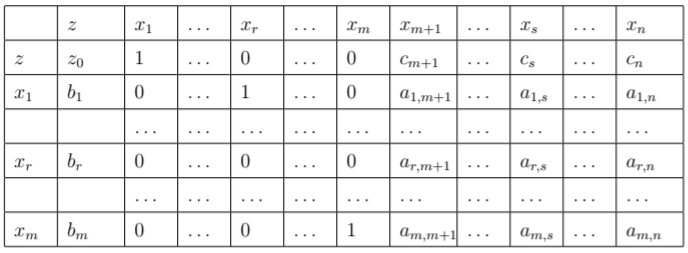
\includegraphics[width=0.5\textwidth]{table}
    \caption{Возможный вид симплекс-таблицы}
    \label{fig:proof1}
\end{figure}

\underline{Алгоритм}
\begin{enumerate}
	\item Составим упорядоченный вектор индексов базисных векторов $B[M]$, где $i$-ый индекс - индекс переменной, которой соответствует столбец $(0\;...\;0\;1\;0\;...\;0)^T$ в матрице коэффициентов с 1 на $i$-й позиции
	
	\item Если $c[N]\geq0$, то решение задачи найдено: $x[N \backslash I[M]]=0$, $x[I[M]]=b[M]$. Алгоритм заканчивает работу
	
	\item Выберем переменную для ввода в базис\\
	Воспользуемся правилом Бленда: найдем индекс $j$ первого отрицательного элемента в векторе $b[N]$
	
	\item Выберем переменную для вывода из базиса
	\begin{equation}
	i = \arg \min_{i \in M, A[i,j]>0} \frac{b[i]}{A[i,j]}
	\end{equation}
	Если такого индекса нет, то задача неограничена. Алгоритм заканчивает работу
	
	\item Ведущий элемент $d=A[i,j]$ \\
	Разделим строку $A[i,N]$ и элемент вектора $b[i]$ на $d$
	
	\item Пересчитаем матрицу коэффициентов, вектор правых частей ограничений и вектор целевой функции $\forall k \in M \backslash \{i\}$: \\
	$A[k,N] := A[k,N] - A[i,N] \ast A[k,j]$ \\
	$b[k] := b[k] - b[i] \ast A[k,j]$ \\
	$c[N] := c[N] - A[i,N] \ast c[j]$
	
	\item Заменим базисную переменную: \\
	$B[i] = j$ \\
	Перейдем на шаг 2
\end{enumerate}

\subsubsection{Метод искусственного базиса}
Может оказаться, что в матрице $A$ нет базисных линейно независимых столбцов вида $(0\;...\;0\;1\;0\;...\;0)^T$. Тогда начальное решение будем искать с помощью метода искусственного базиса.\\
Рассмотрим вспомогательную задачу:\\
\begin{align*} 
\min_{(x,y)} y[N] \\
A[M,N]x[N]+I[M,M]y[M] &= b[M] \\
c[N]x[N]&=0 \\
x[N] &\geq 0 \\
y[M] &\geq 0
\end{align*}
Решим ее табличным симплекс-методом при условии, что уравнению $c[N]x[N]=0$ не соответствует базисная переменная. То есть на этапе 4 при выборе индекса $i$ это уравнение не учитывается, а на этапе 6 оно пересчитывается, как строки матрицы $A$.\\
\begin{itemize}
	\item Если значение целевой функции после решения меньше нуля, то исходная задача не имеет решения, алгоритм заканчивает работу
	\item Если значение целевой функции равно нулю, то решим исходную задачу с пересчитанными векторами $A$, $b$ и $c$ после работы табличного симплекс-метода с вспомогательной задачей.
\end{itemize}

\subsection{Построение двойственной задачей}
Пусть дана задача ЛП в общем виде:
\begin{align*} 
\min_x c^T[N]x[N] \\
A[M_1,N]x[N]&\geq b[M_1] \\
A[M_2,N]x[N]&=b[M_2] \\
x[N_1]&\geq 0
\end{align*}
Тогда двойственная задача будет иметь вид:
\begin{align*} 
\max_y b^T[M]y[M] \\
A^T[N_1,M]y[M] &\leq c[N_1] \\
A^T[N_2,M]y[M] &= c[N_2] \\
y[M_1]&\geq 0
\end{align*}

\section{Исследование применимости метода}
Приведем задачу к каноническому виду. Получим:
\begin{align*} 
	\overline{A}&=
		\begin{pmatrix} 
			1 & 4 & 0 & -7 & 12 & -12 & -1 & 0 \\ 
			 -3 & -10 & 27 & -9 & -3 & 3 & 0 & -1 \\ 
			 0 & 0 & 13 & -4 & 8 & -8 & 0 & 0 \\ 
			 3 & 1 & -3 & -8 & 0 & 0 & 0 & 0 \\ 
			 9 & 3 & 11 & -4 & 9 & -9 & 0 & 0
		\end{pmatrix}\\
	\overline{b}^T&=
		\begin{pmatrix} 
			-296 &
			 -1115 & 
			 -261 & 
			 -518 & 
			 -92
		\end{pmatrix} \\
	\overline{c}&=
		\begin{pmatrix} 
			 11 & 
			 3 & 
			 5 & 
			 7 & 
			 -1 &
			 1 &
			 0 &
			 0
		\end{pmatrix}
\end{align*} 
Условия применения симплекс-метода выполнены:
\begin{itemize}
	\item $m = 5$, $n=8$ \\
	$m < n$
	
	\item rank $\overline{A}=5=m$
\end{itemize}
Кроме того, множество допустимых значений $x$ не пусто. $x^T=
	\begin{pmatrix} 
		 -2 &
		 1 &
		 56 & 
		 3 &
		 71
	\end{pmatrix} \in S$

\section{Результаты решения}
\subsection{Симплекс-метод}
Симплекс-методом было получено следующее решение:\\
$\overline{x}^T=
	\begin{pmatrix} 
		 3.20408163 &
		 3.41439909 &
		 45.02210884 & 
		 0 &
		 71.65816327
	\end{pmatrix}$\\
Значение целевой функции при этом равно $671.0277777777776$

\subsection{Двойственная задача}
Двойственная задача в общем виде имеет следующий вид:
\begin{align*} 
	\max_y c^T \ast y \\
	A_{\geq}&=
		\begin{pmatrix} 
			-1 & 3 & 0 & -3 & -9 \\ 
			-4 & 10 & 0 & -1 & -3 \\ 
			0 & -27 & -13 & 3 & -11 \\ 
			7 & 9 & 4 & 8 & 4
		\end{pmatrix}\\
	A_{=}&=
		\begin{pmatrix} 
			12 & -3 & 8 & 0 & 9
		\end{pmatrix}\\
	b_{\geq}^T&=
		\begin{pmatrix} 
			-11 & 
			 -3 & 
			 -5 & 
			 -7
		\end{pmatrix} \\
	b_{=}^T&= -1\\
	c^T&=
		\begin{pmatrix} 
			 296 & 1115 & 261 & 518 &  92
		\end{pmatrix}		
\end{align*} 

Симплекс-методом было получено следующее решение:\\
$\overline{y}^T=
	\begin{pmatrix} 
		 0 & 0.07407407 & -1.80555556 & -0.81481481 & 1.51851852
	\end{pmatrix}$\\
Значение целевой функции при этом равно $671.0277777777777$

\subsection{Табличный симплекс-метод}
Табличным симплекс-методом было получено следующее решение:\\
$\overline{x}^T=
	\begin{pmatrix} 
		 3.20408163 &
		 3.41439909 &
		 45.02210884 & 
		 0 &
		 71.65816327
	\end{pmatrix}$\\
Значение целевой функции при этом равно $671.0277777777776$

\section{Обоснование достоверности полученного результата}
\underline{Теорема}\\
Для того, чтобы $\overline{x}[N]$ была оптимальной точкой в задаче ЛП в общем виде, необходимо и достаточно, чтобы $\exists \overline{y}[M]$ такой, что $ \overline{y}[M_1]\geq0$ и функция Лагранжа
\begin{equation*}
\psi(x,y)=c^T[N]x[N]+y^T[M](b[M]-A[M,N]x[N])
\end{equation*}
на множествах $x[N_1]\geq0$, $y[M_1]\geq0$ имела седловую точку $(\overline{x}[N],\overline{y}[M])$.\\
\\
Проверим, являются ли наши решения прямой и двойственной задач седловой точкой функции Лагранжа. Для этого убедимся, что если значения целевых функций прямой задачи и двойственной равны, то решения составляют седловую точку.\\
\begin{equation*}
\psi^{\ast}(x)=\text{sup}_{\forall y\geq0}\psi(x,y)
\end{equation*}
\begin{equation*}
\psi_{\ast}(y)=\text{inf}_{\forall x \in S}\psi(x,y)
\end{equation*}
Задача $\min_{x[N_1]\geq0} \psi^{\ast}(x)$ эквивалентна общей задаче ЛП, которую мы решали. \\
Задача $\max_{y[M_1]\geq0} \psi_{\ast}(y)$ эквивалентна двойственной задаче ЛП, которую мы решали.\\
\\
Были найдены допустимые решения $\overline{x}[N]$ и $\overline{y}[M]$ при которых значения целевых функций обеих задач совпали:
\begin{equation*}
\psi_{\ast}(\overline{y})=\psi^{\ast}(\overline{x})
\end{equation*}
Запишем следующие неравенства:
\begin{align*}
\psi(x,y)\leq \psi^{\ast}(x) &\implies \psi(\overline{x},y)\leq \psi^{\ast}(\overline{x}) \\
\psi_{\ast}(y)\leq \psi(x,y),\forall x \in S &\implies \psi_{\ast}(y)\leq \psi(\overline{x},y) \implies \psi_{\ast}(\overline{y})\leq \psi(\overline{x},\overline{y})
\end{align*} 
Значит:
\begin{equation*}
\psi(\overline{x},y)\leq \psi^{\ast}(\overline{x})=\psi_{\ast}(\overline{y})\leq \psi(\overline{x},\overline{y})
\end{equation*}
Аналогично получим, что:
\begin{equation*}
\psi(\overline{x},\overline{y})\leq \psi^{\ast}(\overline{x})=\psi_{\ast}(\overline{y})\leq \psi(x,\overline{y})
\end{equation*}
Это и есть определение седловой точки.\\
Значит, по теореме $\overline{x}[N]$ является оптимальной точкой.



\end{document}